% Template created by Markus Haug <mh@haugmarkus.com>
% Credits: Markus Haug and the template contributors.
% Feel free to share and modify this template, but please give credit where it's due.
%!TEX program = lualatex

\documentclass{article}[11pt, a4paper, oneside, ngerman]


%% 
%% Pakete & Formalia
%%
\usepackage[ngerman]{babel} % neue deutsche Trennungsregeln, etc
\usepackage[hidelinks]{hyperref} % Hyperlinks ohne Umrandungen
\usepackage{setspace} % Abstände zwischen Absätzen
\usepackage[left=2cm, right=2cm, top=2cm, bottom=2cm]{geometry} % Seitenränder
\onehalfspacing % 1,5 Zeilenabstand
\usepackage{lipsum}  % Dummy-Texte
\usepackage{titlesec} % define size for section headings
\usepackage[nohyperlinks, printonlyused]{acronym} % Abkürzungen
\usepackage[utf8]{inputenc} % korrekte Darstellung von Umlauten
\usepackage[T1]{fontenc} % enable hyphenation for languages with accented characters

%% Schriftarten und -größen
\usepackage{fontspec}
\setmainfont{Arial} % Hauptfont Arial (lualatex oder xelatex benötigt)
\titleformat{\section}{\normalfont\fontsize{12pt}{1.5}\bfseries}{\thesection}{1em}{} % Überschriften 1pt größer
\titleformat{\subsection}{\normalfont\fontsize{12pt}{1.5}\bfseries}{\thesubsection}{1em}{} % Überschriften 1pt größer
\titleformat{\subsubsection}{\normalfont\fontsize{12pt}{1.5}\bfseries}{\thesubsubsection}{1em}{} % Überschriften 1pt größer
\def\UrlFont{\rm} % Print URLs not in Typewriter Font
\renewcommand{\footnotesize}{\fontsize{10pt}{1.5pt}\selectfont}

% automatischens Einrücken von Absätzen verhindern
\usepackage{changepage}
\setlength{\parindent}{0pt}
% 6pt Abstand nur zwischen Absätzen
\setlength{\parskip}{6pt}{}

% Leerseite ohne Seitennummer, nächste Seite rechts
\newcommand{\blankpage}{
 \clearpage{\pagestyle{empty}\cleardoublepage}
}

% Grafiken einbinden
\usepackage{graphicx}      
% center images and tables 
\makeatletter
\g@addto@macro\@floatboxreset\centering
\makeatother


%% Informationen für die PDF-Datei
% TODO: Update this!
\hypersetup{
 pdfauthor={Dein Name},
 pdftitle={Mein Titel}, %% Titel der PDF-Datei
  pdfsubject={Fallstudie - IU Wissdoc Template},
 pdfkeywords={},
 pdfcreator={lualatex},
 pdfproducer={lualatex - Template by Markus Haug},
}

%%
%% Bibliographie & Sondereinstellungen
%%
\usepackage[babel]{csquotes}
\usepackage[backend=biber, style=apa, pagetracker, ibidtracker=constrict, apamaxprtauth=20 ]{biblatex}

% Remove Comma after second to last author and ampersand
% https://tex.stackexchange.com/questions/670888/biblatex-apa-7-modification
\makeatletter
\renewcommand*{\apablx@ifrevnameappcomma}{\@secondoftwo}
\makeatother

\DefineBibliographyExtras{ngerman}{%
  \renewcommand*{\finalandcomma}{}%
}

%% Verwendung von "ebenda (ebd.)", wenn eine Quelle hintereinander zitiert wird. 
%% Dies ist nicht im Standard von APA definiert und muss somit explizit aktiviert werden.
%% https://tex.stackexchange.com/questions/449249/getting-ibid-for-apa-style-citations-from-biblatex

\makeatletter
\providecommand*{\mkibid}[1]{#1}

\newbibmacro*{cite:ibid}{%
  \printtext[bibhyperref]{\bibstring[\mkibid]{ibidem}}}

\renewbibmacro*{cite}{%
  \ifthenelse{\ifciteibid\AND\NOT\iffirstonpage}
    {\usebibmacro{cite:ibid}}
    {\iffieldequals{namehash}{\cbx@lasthash}
   % Multiple cites in one command
      {\setunit{\compcitedelim}%
       \usebibmacro{cite:plabelyear+extradate}}%
   % Single cite
      {\ifnameundef{labelname}
   % No author/editor
        {\usebibmacro{cite:noname}%
          \setunit{\printdelim{nameyeardelim}}%
          \usebibmacro{cite:plabelyear+extradate}%
          \savefield{namehash}{\cbx@lasthash}}
   % Normal cite
        {\ifnameundef{shortauthor}
          {\printnames{labelname}}%
          {\cbx@apa@ifnamesaved
            {\printnames{shortauthor}}
            {\printnames[labelname]{author}%
             \addspace\printnames[sabrackets]{shortauthor}}}%
          \setunit{\printdelim{nameyeardelim}}%
         \usebibmacro{cite:plabelyear+extradate}%
         \savefield{namehash}{\cbx@lasthash}}}}%
   \setunit{\multicitedelim}}

\renewbibmacro*{textcite}{%
  \iffieldequals{namehash}{\cbx@lasthash}
% Compact cite - more than one thing for same author
    {\setunit{\compcitedelim}%
     \usebibmacro{cite:plabelyear+extradate}}
% New cite
    {\ifbool{cbx:parens}
       {\bibcloseparen\global\boolfalse{cbx:parens}}
       {}%
     \setunit{\textcitedelim}%
     \ifnameundef{labelname}
     % No author/editor
       {\iffieldundef{shorthand}%
    % Cite using title
         {\usebibmacro{cite:noname}%
          \setunit{\global\booltrue{cbx:parens}%
                   \printdelim{nonameyeardelim}%
                   \bibopenparen}%
          \usebibmacro{cite:plabelyear+extradate}}
    % Cite using shorthand
         {\usebibmacro{cite:shorthand}}}
  % Normal cite with author/editor
  % Normal full cite
       {\ifnameundef{shortauthor}%
    % Normal full cite
         {\printnames{labelname}}
    % Cite using short author
         {\cbx@apa@ifnamesaved
           {\printnames{shortauthor}}
           {\printnames[labelname]{author}}}%
  % Year
        \setunit{\global\booltrue{cbx:parens}%
                 \printdelim{nameyeardelim}%
                 \bibopenparen}%
  % Put the shortauthor inside the year brackets if necessary
        \ifnameundef{shortauthor}
         {}
         {\cbx@apa@ifnamesaved
           {}
           {\printnames{shortauthor}%
            \setunit{\printdelim{innernameyeardelim}}}}%
  % Print prenote (belongs to first cite)
        \ifnumequal{\value{citecount}}{1}
           {\usebibmacro{prenote}}
           {}%
  % Actual year printing
        \ifthenelse{\ifciteibid\AND\NOT\iffirstonpage}
          {\usebibmacro{cite:ibid}}
          {\usebibmacro{cite:plabelyear+extradate}}%
  % Save name hash for checks later
        \savefield{namehash}{\cbx@lasthash}}%
    \stepcounter{textcitecount}}}
\makeatother


%% Bibliographie einbinden
\addbibresource{references.bib} % your bib file
\addbibresource{biblatex-examples.bib} % TODO: remove sample bib 


%% ++++++++++++++++++++++++++++++++++++++++++
%% Dokument
%% ++++++++++++++++++++++++++++++++++++++++++
\begin{document}

\pagenumbering{Roman} % Uppercase Roman numerals
% \pagenumbering{gobble} % switch off page numbering
%% Titelseite
\def\usesf{}
\let\usesf\sffamily % diese Zeile auskommentieren für normalen TeX Font

\newsavebox{\Tutorin}
\savebox{\Tutorin}{<Name des Tutors>}


\setlength{\unitlength}{1pt}

\begin{titlepage}
%\vspace*{-39pt}\hspace*{300pt}\includegraphics[width=.27\paperwidth]{logos/IOSB}
\vspace{-39pt}\hspace*{300pt}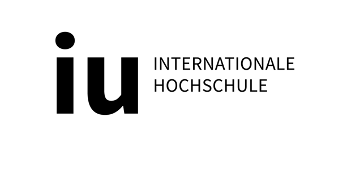
\includegraphics[width=.21\paperwidth]{logos/IU.png}

\begin{center}
\hbox{}
\vfill
{\usesf}
{\huge\bfseries Meine Fallstudie \par}
\vskip 1.8cm
Fallstudie\\[2mm]
\vskip 1cm

{\large\bfseries Markus Haug (<Matrikelnummer>)\\}
\vskip 1.2cm
Wirtschaftsinformatik (B.Sc.)\\
% im Modul\\
ABCDF01 - Kurskürzel\\
\today % TODO: Check Datum
\vskip 3cm
\begin{tabular}{p{3cm}l}
Tutorin: & \usebox{\Tutorin} \\
\end{tabular}
\vfill
\end{center}

\end{titlepage}
%% Titelseite Ende


%%% Local Variables:
%%% mode: latex
%%% TeX-master: "thesis"
%%% End:
 % Titelblatt

\newpage
%% ++++++++++++++++++++++++++++++++++++++++++
%% Verzeichnisse
%% ++++++++++++++++++++++++++++++++++++++++++
\stepcounter{page}
\setcounter{tocdepth}{3}
\tableofcontents % Inhaltsverzeichnis

\blankpage
\phantomsection
\addcontentsline{toc}{section}{Abbildungsverzeichnis}
\listoffigures % Abbildungsverzeichnis



% TODO: Check if needed
%\blankpage
%\listoftables % Tabellenverzeichnis
%\addcontentsline{toc}{section}{Tabellenverzeichnis} 

\blankpage
\section*{Abkürzungsverzeichnis}
\addcontentsline{toc}{section}{Abkürzungsverzeichnis}

% TODO: Check acronyms!
\begin{acronym}
\acro{iu}[IU]{IU Internationale Hochschule}
\end{acronym}
%\label{last-roman-page}% Save last page of this chapter

%% ++++++++++++++++++++++++++++++++++++++++++
%% Hauptteil
%% ++++++++++++++++++++++++++++++++++++++++++
\blankpage
\pagenumbering{arabic}
\section{Einleitung}

Bis zum Jahr 2030 wird der weltweite Fachkräftemangel voraussichtlich insgesamt 82,5 Millionen Fachkräfte umfassen. Insbesondere in der IT-Branche fehlen zahlreiche talentierte Fachkräfte, vor allem Entwickler, um die digitale Transformation eines Unternehmens mit vorantreiben zu können (\cite{grid_dynamics_holdings_inc_software_2022}). Dadurch, dass es für Unternehmen immer schwieriger wird, talentierte professionelle Entwickler einzustellen, stellt dies eines der größten Risiken für Unternehmen dar (\cite{gartner_inc_gartner_2019}).

In den letzten Jahren wurden vermehrt Entwicklungsplattformen auf den Markt gebracht, die sich hauptsächlich dadurch auszeichnen, Anwendungen oder Prozesse mit visuellen Werkzeugen zu erstellen. 
Der Einsatz dieser sogenannten \ac{lcnc}-Plattformen erfordert oft sehr geringe Programmierkenntnisse (\cite[070007-2]{sahinaslan_low-code_2021}). Dies ermöglicht wiederum den Einsatz außerhalb der IT-Abteilung, wodurch erfahrene Anwender aus den Fachabteilungen, Anwendungen selbst erstellen oder Prozesse automatisieren können (\cite[101]{lebens_rise_2021}). 

Diese Anwender werden auch „Citizen Developer“ genannt. Gartner, Inc. (\cite*[][]{gartner_inc_gartner_nodate}) definiert diese im “Information Technology Gartner Glossary” wie folgt:

\begin{adjustwidth}{1.27cm}{0cm}
A citizen developer is an employee who creates application capabilities for consumption by themselves or others, using tools that are not actively forbidden by IT or business units. 
A citizen developer is a persona, not a title or targeted role. They report to a business unit or function other than IT.
\end{adjustwidth}

Durch die aktive Einbeziehung von Citizen Developers in die digitale Transformation entstehen neue Potenziale, aber auch Herausforderungen. 
Folgende Forschungsfragen werden im Rahmen dieser Arbeit beantwortet: 

\begin{itemize}
\item Welche Potenziale eröffnen sich für Unternehmen durch die Nutzung von \ac{lcnc}-Plattformen und wie wirkt sich der Einsatz auf den Mangel von Entwicklern aus? 
\item Welche Maßnahmen sind erforderlich, um die mit \ac{lcnc}-Plattformen einhergehenden Herausforderungen zu bewältigen? 
\end{itemize}

Die Auswirkungen des Einsatzes von \ac{lcnc}-Plattformen auf den Mangel von Entwicklern werden quantitativ erforscht. Darüber hinaus werden IT-Experten und Führungskräfte im Rahmen eines Interviews befragt, welches tiefere Einblicke in die Potenziale und notwendigen Maßnahmen zur Bewältigung potenzieller Herausforderungen in Unternehmen gewähren. Die Ergebnisse werden anschließend ausgewertet und präsentiert. Zum Schluss werden die wichtigsten Inhalte und Erkenntnisse zusammengefasst und es wird ein Ausblick auf mögliche weitere Forschungsthemen gegeben.

\phantomsection
\addtocounter{subsubsection}{1}
\addcontentsline{toc}{subsection}{Problemstellung}

Die Digitalisierung ist in aller Munde. Unternehmen müssen sich immer mehr anpassen, um mit der Konkurrenz Schritt halten zu können.
 % Einleitung
\section{Hauptteil}

\lipsum[1]

\subsection{Titel 1}

Erstes Zitat ist normal mit \parencite[12]{sigfridsson}, das zweite mit "ebenda (ebd.") 
\parencite[78-79]{sigfridsson}, aber nach einer neuen Quelle \parencite[30]{geer} ist es wieder normal \parencite[20]{sigfridsson}.

Dieser Absatz nutzt wieder eine neue Quelle \parencite{nussbaum}.

First citation should be normal \parencite[11]{sigfridsson}, second time with ibidem
\parencite[95]{sigfridsson}, but after a second citation \parencite[282]{geer} it should appear as usual \parencite[2]{sigfridsson}.

\subsection{Titel 2}

Im Abbildung \ref*{fig:logo_iu} in Abschnitt \ref*{pos:logo_iu} wird das Logo der \ac{iu} dargestellt:

\begin{figure}[ht!]
    \label{pos:logo_iu}
    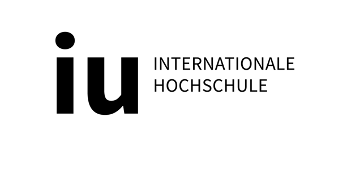
\includegraphics[scale=0.35]{logos/IU.png}
    \caption[Logo der \acs{iu}]{Logo der \ac{iu}}{Quelle: https://iu.de}
    \label{fig:logo_iu}
\end{figure}


\lipsum[7-8]  % Hauptteil
\section{Schluss}

\lipsum[4-5]
  % Schluss

%% ++++++++++++++++++++++++++++++++++++++++++
%% Literatur
%% ++++++++++++++++++++++++++++++++++++++++++
\blankpage

\phantomsection
\pagenumbering{Roman} % Uppercase Roman numerals
\setcounter{page}{5}
% set bibliography name
\renewcommand{\bibname}{Literaturverzeichnis}
\addcontentsline{toc}{section}{\bibname}
% \nocite{*} % nur angeben, wenn auch nicht im Text zitierte Quellen 

\begin{flushleft}

\printbibliography[title=\bibname]
\end{flushleft}

% %% ++++++++++++++++++++++++++++++++++++++++++
% %% Anhang
% %% ++++++++++++++++++++++++++++++++++++++++++
% \blankpage
% \appendix
% \section{Anhang}

\lipsum[1-2] % Anhang % TODO: Add Appendix?

\end{document}

